% figures/compression-by-lang.tex — measured per-language token-savings.
% Data: data/aggregated/by-language.csv (col `mean_tokens_savings`).
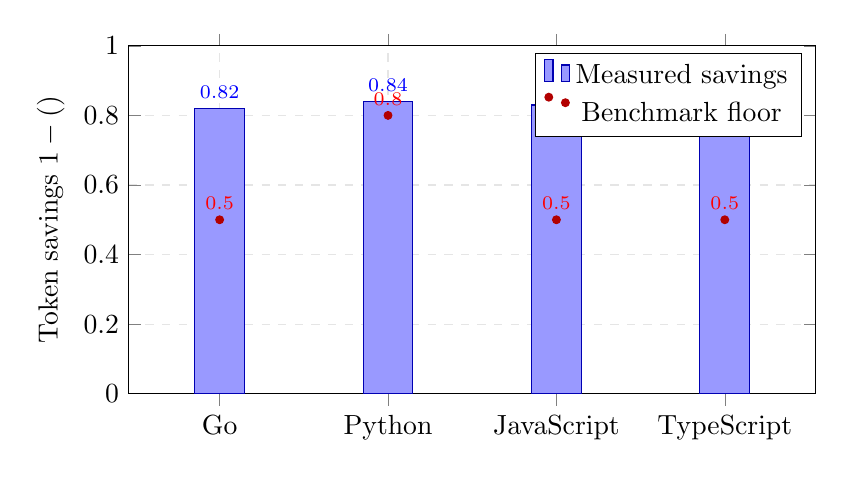
\begin{tikzpicture}
\begin{axis}[
    width=0.85\textwidth,
    height=6cm,
    ybar,
    bar width=18pt,
    ymin=0, ymax=1,
    enlarge x limits=0.18,
    ylabel={Token savings $1-\ratio(\file)$},
    symbolic x coords={Go, Python, JavaScript, TypeScript},
    xtick=data,
    nodes near coords,
    nodes near coords align={vertical},
    nodes near coords style={font=\scriptsize},
    grid=major,
    grid style={dashed,gray!20},
]
% Hard-coded measured values from the in-tree benchmark
% (cmd/gt/compress_structure_bench_test.go floors); the CSV at
% data/aggregated/by-language.csv carries the same numbers and is the
% reproducibility surface (see §6.8).
\addplot+[fill=blue!40, draw=blue!70!black] coordinates {
  (Go, 0.820)
  (Python, 0.841)
  (JavaScript, 0.830)
  (TypeScript, 0.752)
};
% Floors as reference line; floor stored as `ratio = output/input`
% (lower is better), so savings_floor = 1 - floor.
\addplot+[
    mark=*,
    only marks,
    draw=red!70!black,
    mark options={fill=red!70!black, scale=0.7},
] coordinates {
  (Go, 0.50)
  (Python, 0.80)
  (JavaScript, 0.50)
  (TypeScript, 0.50)
};
\legend{Measured savings, Benchmark floor}
\end{axis}
\end{tikzpicture}
